\subsection{Political books}

The goal here is to 
determine whether the authors' political affiliations are a good predictor 
of the overall network structure. We choose to partition the network into $B=3$ communities as we only have this many distinct values for political affiliation (conservative, liberal or neutral).
%
\begin{figure}[!h]
	\centering
	\begin{subfigure}[t]{0.452\linewidth}
		\centering
		\vskip 0pt
		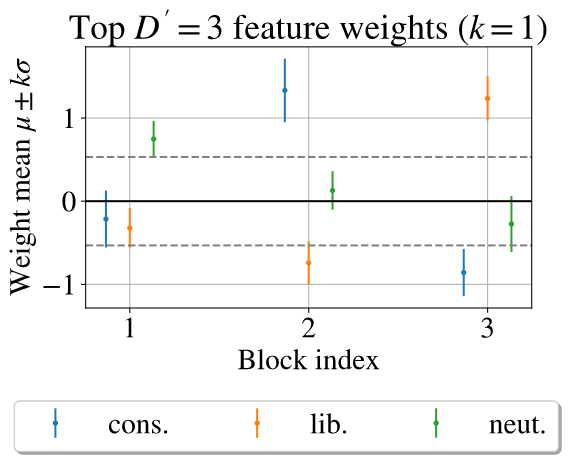
\includegraphics[width=\linewidth]{polbooks-null-1}
		\caption{$\theta$-samples. Dotted line is $\pm c^*$.}
		\label{fig:polbooks-null}
	\end{subfigure}
	\begin{subfigure}[t]{0.45\linewidth}
		\centering
		\vskip 0pt
		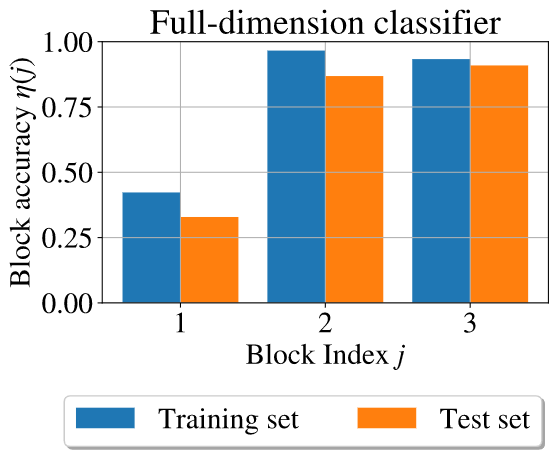
\includegraphics[width=\linewidth]{polbooks-accuracy-1}
		\caption{Per-block accuracy $\eta(j)$.}
		\label{fig:polbooks-accuracy}
	\end{subfigure}
	\caption{Political books dataset.}
	\label{fig:polbooks}
\end{figure}

From Figure~\ref{fig:polbooks-null} we see that all 3 blocks have a distinct political affiliation as their largest positive component. 
This strongly indicates that political affiliation is indeed the axis 
which best predicts the 3-way natural partition of the graph into blocks. 
Furthermore, in Table~\ref{tab:results} we see that the training and test losses 
are very similar and both are low in magnitude. This provides further evidence 
to the claim that political affiliation is a very appropriate explanatory 
variable for the overall network structure.

However, from Figure~\ref{fig:polbooks-accuracy} we see that block 1 has low accuracy. 
This suggests that detected block 1 is not solely composed of ``neutral" books but also 
contains some ``liberal" and ``conservative" authors. Indeed, by examining 
Figure~\ref{fig:polbooks-graph} we see that block 1 is effectively a buffer between 
blocks 2 and 3; there are very few edges between blocks 2 and 3. It is therefore not 
surprising that some books from either side leak into block 1.
Perhaps, the three distinct categories (``conservative", ``liberal", ``neutral") are 
too coarse a measure of political affiliation; it may be the case that the nominally 
``conservative" books found in block 1 are in fact more centre-right. 
In the absence of more granular labels, we cannot test this hypothesis. 
Nevertheless, political affiliation encoded as 3 distinct labels 
remains a fantastic predictor of network structure.

\subsection{Primary school dynamic contacts}

We choose the number of communities $B=10$, in line with the total number of 
school classes. As before, we sample the block-generator parameters $\theta$ and 
employ the dimensionality reduction technique 
of Section~\ref{sec:dim-reduction},
with standard deviation multiplier $k=1$ to pick out the top $D'=10$ features. 
We then plot the weights for the resulting features $d \in \Dcal'$ 
in Figure~\ref{fig:school-null}. It is rather obvious
that only the pupils' class memberships (1A-5B) have remained
significant;
gender and teacher/student status have been discarded,
meaning that these are not good predictors of overall macro-structure.
%
\begin{figure}[!h]
	\centering
	\begin{subfigure}[t]{0.45\linewidth}
		\centering
		\imagebox{0.8\linewidth}{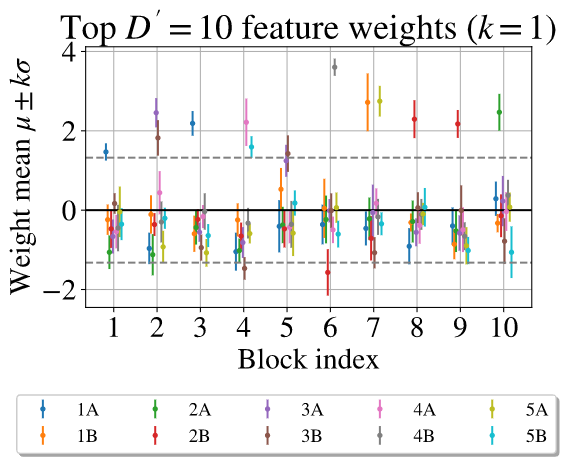
\includegraphics[width=\linewidth]{school-null-1}}
		\caption{$\theta$-samples. Dotted line is $\pm c^*$.}
		\label{fig:school-null}
	\end{subfigure}
	\begin{subfigure}[t]{0.45\linewidth}
		\centering
		\imagebox{0.8\linewidth}{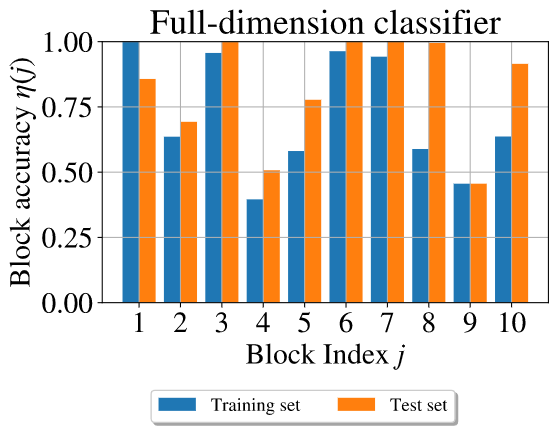
\includegraphics[width=\linewidth]{school-accuracy-1}}
		\caption{Per-block accuracy $\eta(j)$.}
		\label{fig:school-accuracy}
	\end{subfigure}
	\caption{Primary school dynamic contacts dataset.}
	\label{fig:school}
\end{figure}

The vast majority of blocks are composed of a single class. 
However, some blocks have two comparably strong classes as their predictors. 
For example, blocks 2 and 5 both contain classes 3A and 3B as their 2 best predictors. 
This suggests that the social divide between classes is less pronounced 
for pupils in year 3. Conversely, some classes are found to extend over two 
detected blocks (class 2B spans blocks 8 and 9) but we do 
not have a feature which explains the division. The most surprising block 
is number 7, which has comparable weightings for classes 5A and 1B. 
Perhaps there was a joint event between those two classes on the day 
the data were collected.

Figure~\ref{fig:school-accuracy} shows excellent accuracy for the majority of blocks. In fact the only blocks with low accuracy are those that have a school-class span two blocks such that we cannot reliably distinguish between the two. This is much more pronounced when we apply hard classification rather than the soft cross-entropy loss. Indeed block 1 has low accuracy because class 1A has a higher weight component for block 3 than it does for block 1. As we use hard classification to compute accuracy, vertices belonging to class 1A are predicted to belong to block 3. A similar effect is seen in block 5 which often loses out to block 2. The same can be said of blocks 8 and 9. However, in this case the weights for class 2B are very similar -- thus explaining the roughly evenly split accuracy for blocks 8 and 9.

\subsection{Facebook egonet}

We choose $B=10$ and $D'=10$ for this experiment. The selected features 
(Figure~\ref{fig:fb-null}) are those that best explain the high-level 
community structure. The majority of them are education related. 
Nevertheless, for $D'=10$ we only have good explanations for the makeup 
of some of the detected blocks; several blocks in 
Figure~\ref{fig:fb-null} do not have high-magnitude components for $D'=10$. This is further emphasised by the disparate accuracies in Figure~\ref{fig:fb-accuracy}. Nevertheless, observe that the accuracy is only high for blocks that contain high magnitude weights. The only exception to this rule is block 9 which nonetheless may have high magnitude weights just below the cut-off $c^*$.
%
\begin{figure}[!h]
	\centering
	\begin{subfigure}[t]{0.45\linewidth}
		\centering
		\imagebox{0.9\linewidth}{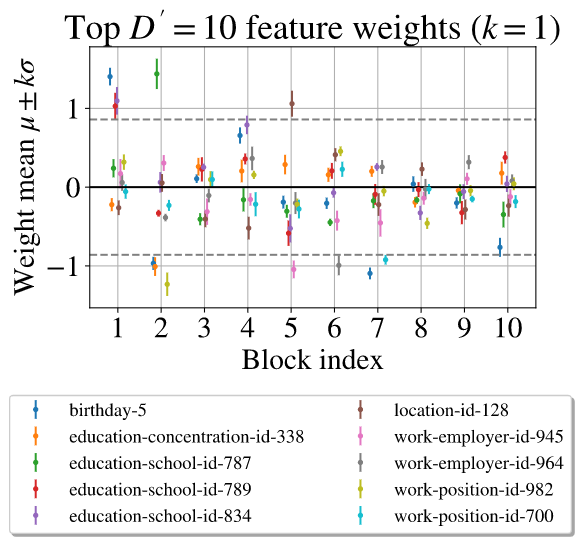
\includegraphics[width=\linewidth]{fb-null-1}}
		\caption{$\theta$-samples. Dotted line is $\pm c^*$.}
		\label{fig:fb-null}
	\end{subfigure}
	\begin{subfigure}[t]{0.45\linewidth}
		\centering
		\imagebox{0.9\linewidth}{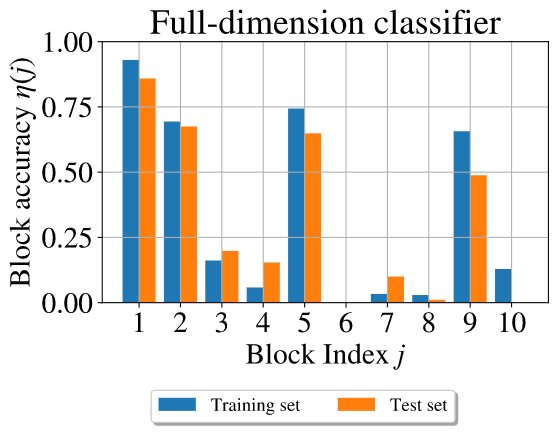
\includegraphics[width=\linewidth]{fb-accuracy-1}}
		\caption{Per-block accuracy $\eta(j)$.}
		\label{fig:fb-accuracy}
	\end{subfigure}
	\caption{Facebook egonet dataset.}
	\label{fig:fb}
\end{figure}

When the feature dimension is very large, it becomes increasingly likely that 
a particular feature may uniquely identify a small set of nodes. If these nodes 
are all part of the same community, then the classifier may overfit for that 
particular parameter. The regularisation term imposed by the prior goes some 
way towards alleviating this problem. Nevertheless, we see in 
Figure~\ref{fig:fb-null} that the feature \verb*|birthday-5| has a very 
high weight as it relates to block 1 -- but it is highly unlikely
that birthdays determine graphical structure. This issue could have been alleviated by 
choosing $\Xcal=\{-1, +1\}$ such that having a feature turned off supports excluding 
a vertex from the block. However, Figure~\ref{fig:fb-null} demonstrates why we made 
the deliberate choice $\Xcal=\{0,1\}$. 
Because of the choice $\Xcal=\{0,1\}$, block 1 is allowed to contain 3 distinct feature 
categories rather than just one. We accept this trade-off: risking spurious high magnitude 
components (e.g. \verb*|birthday-5|) for the benefit of allowing a top-level block to span 
multiple feature-groups. Nevertheless, one would have to apply a hierarchical approach 
to subdivide each top-level block into sub-blocks to test whether the constituent 
feature-groups determine structure at the lower-level.